\documentclass{article}
\usepackage[utf8]{inputenc}
\usepackage{geometry}
\usepackage{pdfpages}
\usepackage{filecontents}
\graphicspath{{images/}}
\geometry{
	a4paper,
	total={170mm,257mm},
	left=20mm,
	top=20mm,
}
\usepackage{graphicx}
\usepackage{titling}
\usepackage[american,RPvoltages]{circuiTikz}
\usepackage{tikz, tikz-cd}
\usepackage{pgfplots}
\usepackage{siunitx}
\usepackage{float}
\usepackage{enumitem}
\usepackage{amsmath,amsfonts,stmaryrd,amssymb} % Math packages
\usepackage{schemabloc}
\usepackage{tcolorbox}
\title{Diodo con fuente de AC y fuente de DC}
\author{Rodrigo}
\date{Agosto 2024}

\usepackage{fancyhdr}
\fancypagestyle{plain}{%  the preset of fancyhdr 
	\fancyhf{} % clear all header and footer fields
	\fancyfoot[L]{\thedate}
	\fancyhead[L]{Diseño con OpAmp}
	\fancyhead[R]{\theauthor}
}
\makeatletter
\def\@maketitle{%
	\newpage
	\null
	\vskip 1em%
	\begin{center}%
		\let \footnote \thanks
		{\LARGE \@title \par}%
		\vskip 1em%
		%{\large \@date}%
	\end{center}%
	\par
	\vskip 1em}
\makeatother

\usepackage{lipsum}  
\usepackage{cmbright}

%---------------------------------------------------
\tikzset{flipflop myRS/.style={flipflop,
		 flipflop def={t1=R, t3=S, t6=Q, t4={\ctikztextnot{Q}}, tu={\ctikztextnot{RST}}, nu=1, n4=1 }}
	}
	
\tikzset{flipflop myFFRS/.style={flipflop,
		flipflop def={t1=R, t3=S, t6=Q, t4={\ctikztextnot{Q}}, n4=1 }}
}
%---------------------------------------------------

\makeatletter
\newcommand*{\underarrow}{\def\@underarrow{\relax}\@ifstar{\@@underarrow}{\def\@underarrow{\hidewidth}\@@underarrow}}
\newcommand*{\@@underarrow}[2][]{\underset{\@underarrow\substack{\uparrow\if\relax\detokenize{#1}\relax\else\\#1\fi}\@underarrow}{#2}}

\newcommand*{\overarrow}{\def\@overarrow{\relax}\@ifstar{\@@overarrow}{\def\@overarrow{\hidewidth}\@@overarrow}}
\newcommand*{\@@overarrow}[2][]{\overset{\@overarrow\substack{\if\relax\detokenize{#1}\relax\else#1\\\fi\downarrow}\@overarrow}{#2}}
\makeatother

\begin{document}
	
\maketitle
	
\noindent\begin{tabular}{@{}ll}
Author & \theauthor\\
Chapter &  3 - Switching Diode Circuits \\
Example & 3.3 - pp. 104
\end{tabular}
	
\section*{Problema}
Considere el circuito con diodo que se muetra en la figura 1 el cual contiene una fuente de dc en el lado de la carga la cual puede representar una batería o una fuerza contraelectromotríz (emf) para excitar la armadura en un motor de dc. Grafique las formas de onda para $i_o, v_D$ y $v_o$. Asuma que $V_s = V_m \sin(\omega t) \, V$

\begin{figure}[H]
	\centering	
	\begin{tikzpicture}[scale=0.8]
		\def\x{2.1*pi}% scalebar-x at golden ratio of x=1728px
		\def\y{320}% scalebar-y at 90% of height of y=356px
		\ctikzset{bipoles/thickness=4}
		\ctikzset{monopoles/vcc/arrow={Stealth[width=6pt,length=9pt]}}
		\ctikzset{monopoles/vee/arrow={Stealth[width=6pt,length=9pt]}}
		\draw (0,0)++(0,-3) to[sV, l=$v_s$] ++(0,6)
		      to[D, i_=$i_o$, v^=$v_D$] ++(5,0) coordinate (p1)
		      to[R, l_=$R$] ++(0,-3)
		      to[V,l_=$V_{DC}$, invert] ++(0,-3)
		      to[short] ++(-5,0);
		\draw (p1)++(1,0) to[open, v_=$v_O$] ++(0,-6);
		
		\pgfplotsset{width=10cm,height=5cm,compat=1.18}
		
		\begin{axis}[name=plot1,
			xshift=8cm,
			yshift=4cm,
			clip=false,
			axis y line=left,
			axis x line=middle,
			%grid style={line width=.1pt, draw=gray!20},
			%grid=both,
			%minor tick num=1,
			xlabel=$\omega (t)$,
			%ylabel=$v_s$, 
			axis y line= center,
			xmin=0,xmax=2.5*pi,
			ymin=-1,ymax=1.2,
			xtick={0.3,pi,2*pi, 3*pi, 4*pi},
			ytick={1},
			xticklabels={$\,\,\,\,\,\,\,\,\,\alpha_1$,$\,\,\,\,\,\,\,\,\,\,\pi$,$\,\,\,\,\,\,\,\,\,\,2\pi$},
			yticklabels={$V_m$},
			]
			\addplot[smooth, magenta,thick, mark=none, domain=0:\x, samples=500] {sin(deg(x))};
			%\addplot[smooth, magenta,thick, mark=none, domain=0.001:0.002, samples=200] {3000*(x - 0.001)};
			%\addplot[smooth, magenta,thick, mark=none, domain=0.002:0.003, samples=200] {3000*(x - 0.002)};
			\addplot[thick, dashed] coordinates {(0,1) (0.5*pi,1)}; %horizontal1
			\addplot[thick, dashed] coordinates {(0,0.29552) (2.84159,0.29552)}; %horizontal2
			\addplot[color = black, thick, dashed] coordinates {(0.3,0.29552) (0.3,-8.4)}; %vertical2
			\addplot[color = black, thick, dashed] coordinates {(pi-0.3,0.29552) (pi-0.3,-8.4)}; %vertical2
			\addplot[color = black, thick, dashed] coordinates {(pi,0) (pi,-8.4)}; %vertical3
			\addplot[color = black, thick, dashed] coordinates {(2*pi,0) (2*pi,-8.4)}; %vertical4
			\draw[->](2.4, -0.2)--(2.7, -0.05);
			\node[anchor=east] at (axis cs:pi-0.3,-0.3){$\pi - \alpha$};
			\node[left] at(0,1.2){$v_s$};
			\node[left] at(0,0.29552 ){$v(\alpha)$};
		\end{axis}
		
		\begin{axis}[name=plot2,
			xshift=8cm,
			yshift=0cm,
			clip=false,
			axis y line=left,
			axis x line=middle,
			%grid style={line width=.1pt, draw=gray!20},
			%grid=both,
			%minor tick num=1,
			xlabel=$\omega (t)$,
			%ylabel=$v_s$, 
			axis y line= center,
			xmin=0,xmax=2.5*pi,
			ymin=-0.2,ymax=1.2,
			xtick={0.3,pi,2*pi, 3*pi, 4*pi},
			ytick={0.29552, 1},
			xticklabels={$\,\,\,\,\,\,\,\,\,\alpha_1$,$\,\,\,\,\,\,\,\,\,\pi$,$\,\,\,\,\,\,\,\,\,\,2\pi$},
			yticklabels={$V_{DC}$,$V_m$},
			]
			%\addplot[smooth, cyan,thick, mark=none, domain=0:pi, samples=500] {sin(deg(x))};
			\addplot[smooth, magenta,thick, mark=none, domain=0.3:(pi-0.3), samples=500] {sin(deg(x))};
			\addplot[thick, dashed] coordinates {(0,1) (0.5*pi,1)}; %horizontal1
			\addplot[thick, magenta] coordinates {(0,0.29552) (0.3,0.29552)}; %horizontal2
			\addplot[thick, magenta] coordinates {(pi-0.3,0.29552) (2*pi,0.29552)}; %horizontal3
			\draw[->](2.4, -0.2)--(2.7, -0.05);
			\node[anchor=east] at (axis cs:pi-0.3,-0.3){$\pi - \alpha$};
			\node[left] at(0,1.2){$v_O$};
		\end{axis}
		
		\begin{axis}[name=plot2,
			xshift=8cm,
			yshift=-4cm,
			clip=false,
			axis y line=left,
			axis x line=middle,
			%grid style={line width=.1pt, draw=gray!20},
			%grid=both,
			%minor tick num=1,
			xlabel=$\omega (t)$,
			%ylabel=$v_s$, 
			axis y line= center,
			xmin=0,xmax=2.5*pi,
			ymin=-0.2,ymax=1.2,
			xtick={0.3,pi,2*pi, 3*pi, 4*pi},
			ytick={0.70448},
			xticklabels={$\,\,\,\,\,\,\,\,\,\alpha_1$,$\,\,\,\,\,\,\,\,\,\pi$,$\,\,\,\,\,\,\,\,\,\,2\pi$},
			yticklabels={$I_m$},
			]
			%\addplot[smooth, cyan,thick, mark=none, domain=0:pi, samples=500] {sin(deg(x))};
			\addplot[smooth, magenta,thick, mark=none, domain=0.3:(pi-0.3), samples=500] {sin(deg(x)) - 0.29552};
			\addplot[thick, dashed] coordinates {(0,0.70448) (pi/2,0.70448)}; %horizontal1
			\draw[->](2.4, -0.2)--(2.7, -0.05);
			\node[anchor=east] at (axis cs:pi-0.3,-0.3){$\pi - \alpha$};
			\node[left] at(0,1.2){$i_o$};
		\end{axis}
		
		\begin{axis}[name=plot2,
			xshift=8cm,
			yshift=-8cm,
			clip=false,
			axis y line=left,
			axis x line=middle,
			%grid style={line width=.1pt, draw=gray!20},
			%grid=both,
			%minor tick num=1,
			xlabel=$\omega (t)$,
			%ylabel=$v_s$, 
			axis y line= center,
			xmin=0,xmax=2.5*pi,
			ymin=-0.2,ymax=1.2,
			xtick={0.3,pi,2*pi, 3*pi, 4*pi},
			ytick={0.29552, 1},
			xticklabels={$\,\,\,\,\,\,\,\,\,\alpha_1$,$\,\,\,\,\,\,\,\,\,\pi$,$\,\,\,\,\,\,\,\,\,\,2\pi$},
			yticklabels={$V_{DC}$,$V_m$},
			]
			%\addplot[smooth, cyan,thick, mark=none, domain=0:pi, samples=500] {sin(deg(x))};
			\addplot[smooth, magenta,thick, mark=none, domain=0.3:(pi-0.3), samples=500] {sin(deg(x))};
			\addplot[thick, dashed] coordinates {(0,1) (0.5*pi,1)}; %horizontal1
			\addplot[thick, magenta] coordinates {(0,0.29552) (0.3,0.29552)}; %horizontal2
			\addplot[thick, magenta] coordinates {(pi-0.3,0.29552) (2*pi,0.29552)}; %horizontal3
			%\addplot[color = magenta, thick] coordinates {(0.002,3) (0.002,0)}; %vertical2
			%\addplot[color = magenta, thick] coordinates {(0.003,3) (0.003,0)}; %vertical3
			\draw[->](2.4, -0.2)--(2.7, -0.05);
			\node[anchor=east] at (axis cs:pi-0.3,-0.3){$\pi - \alpha$};
			\node[left] at(0,1.2){$v_D$};
		\end{axis}
	\end{tikzpicture}
	\caption{}	
	\label{fig:figura1}
\end{figure}

\subsection*{Solución}
Emplearemos el principio de superposición para encontrar el voltaje de salida $v_o$ en el circuito de la figura 1(a). Asumamos que estamos tratando con un diodo ideal. De acuerdo al circuito de la figura 2(a) se puede ver por inspección que el diodo está polarizado en directa, por lo que voltaje de salida $v_{o_1}$ está dado por

\begin{align}
	v_{o_1} = v_s
\end{align}

\begin{figure}[H]
	\centering	
	\begin{tikzpicture}[scale=0.8]
		\ctikzset{bipoles/thickness=4}
		\ctikzset{monopoles/vcc/arrow={Stealth[width=6pt,length=9pt]}}
		\ctikzset{monopoles/vee/arrow={Stealth[width=6pt,length=9pt]}}
		\draw (0,0) to[sV, l=$v_s$] ++(0,6)
		to[D, v^=$v_D$] ++(5,0) coordinate (p1)
		to[R, l_=$R$, v^=$v_{o_1}$] ++(0,-6)
		to[short] ++(-5,0);
	
		\draw (p1)++(3,0) to[D, v>=$v_D$] ++(5,0) coordinate(p2)
		      to[R] ++(0,-3)
		      to[V, invert, l_=$V_{DC}$] ++(0,-3)
		      to[short] ++(-5,0)
		      to[short] ++(0,6);
		\draw (p2)++(1,0) to[open, v=$v_{o_2}$] ++(0,-6);
		\node[] at(2.5,-1){$(a)\, Fuente \, de \, dc \, desconectada$};
		\node[anchor=west] at(7,-1){$(a)\, Fuente \, de \, ac \, desconectada$};
	\end{tikzpicture}
	\caption{}	
	\label{fig:figura2}
\end{figure}

\noindent Al observar la figura 2(b), notamos que el voltaje en el cátodo está a un potencial superior que la terminal del ánodo, el cual de hecho, está a $\qty{0}{\volt}$, por lo que el diodo se encuntra polarizado en inversa, así el voltaje de salida $v_{o_2}$ está dado por

\begin{align}
	v_{o_2} = V_{DC}
\end{align}

\noindent Al combinar las ecuaciones (1) y (2) obtenemos el voltaje de salida como

\begin{tcolorbox}[colback=red!5!white,colframe=red!75!black,arc=0mm,boxrule=0mm,width=(\linewidth+0.5cm)]
	\begin{equation}
		v_O = v_s + V_{DC} = V_m \sin (\omega t) + V_{DC}
	\end{equation}
\end{tcolorbox}

\noindent El diodo se encenderá cuando $v_D > 0$ el cual ocurrirá en $\omega t = \alpha$, es decir, cuando $v_s(\alpha) = V_{DC}$
\begin{align}
	V_m \sin (\omega t) = V_{DC} \nonumber
\end{align}

\noindent O bien

\begin{tcolorbox}[colback=red!5!white,colframe=red!75!black,arc=0mm,boxrule=0mm,width=(\linewidth+0.5cm)]
	\begin{equation}
		\alpha = \arcsin \left( \frac{V_{DC}}{V_m} \right)
	\end{equation}
\end{tcolorbox}

\noindent Donde

\begin{align}
	\alpha = \omega t
\end{align}

\noindent Durante el intervalo $0 \leq \omega t \leq \alpha$ el diodo se encontrará en estado $off$ y durante el intervalo $\pi - \alpha \leq \omega t \leq \pi$ el diodo se encontrará en estado de $on$. \\

\noindent Con esto presente, el voltaje de salida puede expresarse como:
\begin{equation}
	v_O(t) =  
	\begin{cases}
		V_{DC} \quad & 0 \leq \omega t \leq \alpha\\
		V_m \sin (\omega t) & \alpha \leq \omega t \leq \pi - \alpha \\
		V_{DC} \quad & \pi - \alpha \leq \omega t \leq 2 \pi\\
	\end{cases}\,.
\end{equation}

\noindent Durante el intervalo $\pi - \alpha \leq \omega t \leq 2\pi$ la corriente de salida estará dada por

\begin{tcolorbox}[colback=red!5!white,colframe=red!75!black,arc=0mm,boxrule=0mm,width=(\linewidth+0.5cm)]
	\begin{equation}
		i_O(t) = \frac{v_s - V_{DC}}{R} = \frac{V_m \sin (\omega t) - V_{DC}}{R}
	\end{equation}
\end{tcolorbox}

\noindent O bien

\begin{equation}
	i_O(t) =  
	\begin{cases}
		0 \quad & 0 \leq \omega t \leq \alpha\\
		\frac{v_s - V_{DC}}{R} & \alpha \leq \omega t \leq \pi - \alpha \\
		0 \quad & \pi - \alpha \leq \omega t \leq 2 \pi\\
	\end{cases}\,.
\end{equation}

\noindent El voltaje de salida promedio se puede obtener a partir de la siguiente ecuación 

\begin{align}
	V_{O(av)} = \frac{1}{T} \int_{0}^{T} f(t) d(\omega t)
\end{align}

\noindent Es decir

\begin{align}
	V_{O(av)} = \frac{1}{2\pi} \left[ \int_{0}^{\alpha} {V_{DC} \, d(\omega t)} + \int_{\alpha}^{\pi - \alpha}{V_m \sin (\omega t) \, d(\omega t) } + \int_{\pi - \alpha}^{2\pi}{V_{DC}} \,d(\omega t) \right]
\end{align}

\noindent Desarrollando cada integral por separado obtenemos

\begin{align}
	\int_{0}^{\alpha} {V_{DC} \, d(\omega t)} = \left.{V_{DC} (\omega t)}\right|_{\;0}^{\;\alpha} = \alpha V_{DC}
\end{align}

\begin{align}
	\int_{\alpha}^{\pi - \alpha}{V_m \sin (\omega t) \, d(\omega t) } = -{\left[ V_m \cos (\omega t) \right]} \bigg\rvert_{\alpha}^{\pi - \alpha} = -V_m \cos (\pi - \alpha) + V_m \cos (\alpha)
\end{align}

\noindent Desarrollamos la siguiente identidad trigonométrica

\begin{align}
	\cos(A - B) = \cos A \cos B + \sin A \sin B
\end{align}

\noindent Es decir

\begin{align}
	\cos(\pi - \alpha) = \cos (\pi)  \cos (\alpha) + \sin(\pi) \sin (\alpha)  = (-1)\cos (\alpha)
\end{align}

\noindent Al sustituir (14) en (12) obtenemos

\begin{align}
	\int_{\alpha}^{\pi - \alpha}{V_m \sin (\omega t) \, d(\omega t) } = -V_m \left[ -\cos (\alpha) \right] + V_m \cos (\alpha) = 2V_m \cos (\alpha)
\end{align}

\noindent De la tercera integral obetenemos

\begin{align}
	\int_{\pi - \alpha}^{2\pi}{V_{DC}} \,d(\omega t) = V_{DC} (\omega t)  \bigg\rvert_{\pi - \alpha}^{2\pi} = V_{DC} \left( 2\pi - (\pi - \alpha) \right) = V_{DC} (2\pi - \pi + \alpha) = (\pi + \alpha)V_{DC}
\end{align}

\noindent Al combinar las ecuaciones (11), (15) y (16) en (10) obtenemos

\begin{align}
		V_{O(av)} &= \left( \frac{1}{2\pi} \right)  \left[ \alpha V_{DC} + 2V_m \cos (\alpha) + (\pi + \alpha)V_{DC} \right] \nonumber
\end{align}

\noindent Así, el voltaje de salida promedio para el circuito de la figura 1(a) está dado por


\begin{tcolorbox}[colback=red!5!white,colframe=red!75!black,arc=0mm,boxrule=0mm,width=(\linewidth+0.5cm)]
	\begin{equation}
	V_{O(av)} = \left( \frac{1}{2\pi} \right) \left[ (2 \alpha + \pi)V_{DC} + 2V_m \cos (\alpha) \right]
	\end{equation}
\end{tcolorbox}

\noindent Para calcular el voltaje de salida rms utilizamos la siguiente ecuación

\begin{align}
	V_{rms} = \sqrt{\frac{1}{T} \int_{0}^{T} {f^2 (t) dt}}
\end{align}

\noindent Sustituyendo (18) por los valores en (6) obtenemos

\begin{align}
	\sqrt{\frac{1}{2\pi} \left[ \int_{0}^{\alpha}{V^2_{DC} (\omega t)} + \int_{\alpha}^{\pi - \alpha}{V^2_m \sin^2(\omega t) \, d(\omega t)}  + \int_{\pi - \alpha}^{2\pi}{V^2_{DC} \, d(\omega t)} \right]}
\end{align}

\noindent Al resolver cada una de las integrales obtenemos:

\begin{align}
	\int_{0}^{\alpha}{V^2_{DC} (\omega t)} = V^2_{DC} (\omega t)  \bigg\rvert_{0}^{\alpha} = \alpha V^2_{DC}
\end{align}

\begin{align}
	\int_{\alpha}^{\pi - \alpha}{V^2_m \sin^2(\omega t) \, d(\omega t)} &= V^2_m \int_{\alpha}^{\pi - \alpha}{ \left[  \frac{1}{2} - \frac{1}{2} \cos (2\omega t) \, d(\omega t)\right] } \nonumber \\
	&=V^2_m \left[ \frac{1}{2} (\omega t)\bigg\rvert_{\alpha}^{\pi - \alpha} - \frac{1}{4} \sin (2 \omega t)\bigg\rvert_{\alpha}^{\pi - \alpha}\right] \nonumber \\
	&= V^2_m \left[ \frac{1}{2} (\pi - \alpha - \alpha) - \frac{1}{4}(\sin(2(\pi - \alpha)) - \sin(2\alpha)) \right] \nonumber \\
	&= V^2_m \left[ \frac{1}{2}(\pi - 2\alpha) - \frac{1}{4}( \sin(2\pi - 2\alpha) - \sin ({2\alpha}) ) \right]
\end{align}

\noindent Utilizamos la siguiente identidad trigonométrica 

\begin{align}
	\sin(a - b) &= \sin a \cos b - \cos a \sin b \nonumber \\
	\sin(2\pi - 2\alpha) &= \sin(2\alpha)cos(2\alpha) - \cos(2\pi)\sin(2\alpha) \nonumber \\ 
	&= -\sin(2\alpha) \nonumber
\end{align}

\noindent El resultado de (21) es, por lo tanto

\begin{align}
	\int_{\alpha}^{\pi - \alpha}{V^2_m \sin^2(\omega t) \, d(\omega t)} &= \frac{1}{2}\pi - \alpha - \frac{1}{4}\left[ -\sin(2\alpha) - \sin(2\alpha) \right] \nonumber \\
	&= V^2_m \left[ \frac{1}{2}\pi - \alpha + \frac{1}{4}\sin (2\alpha) + \frac{1}{4}\sin (2\alpha) \right] \nonumber \\
	&= V^2_m \left[ \frac{1}{2}\pi - \alpha + \frac{1}{2} \sin(2 \alpha) \right]
\end{align}

\noindent En cuanto a la tercera integral:

\begin{align}
	\int_{\pi - \alpha}^{2\pi}{V^2_{DC} (\omega t)} &= V^2_{DC} (\omega t)  \bigg\rvert_{\pi - \alpha}^{2\pi} =  V^2_{DC} \left[ 2\pi - (\pi - \alpha) \right] \nonumber \\
	&=  V^2_{DC} \left[ 2\pi - \pi + \alpha \right] \nonumber \\
	&= (\pi + \alpha)V^2_{DC}
\end{align}

\noindent La combinación los resultados de las ecuaciones (20), (22) y (23) en (19) produce

\begin{align}
	V_{o(rms)} = \sqrt{\frac{1}{2\pi} \left[ \alpha V^2_{DC} + (\pi + \alpha)V^2_{DC} + V^2_m \left( \frac{1}{2}\pi - \alpha + \frac{1}{2} \sin 2 \alpha \right)  \right] } \nonumber
\end{align}

\noindent Al reordenar términos obtenemos

\begin{tcolorbox}[colback=red!5!white,colframe=red!75!black,arc=0mm,boxrule=0mm,width=(\linewidth+0.5cm)]
	\begin{equation}
		V_{o(rms)} = \sqrt{\frac{1}{2\pi} \left[ (\pi + 2\alpha)V^2_{DC} + \frac{V^2_m}{2} \left(\pi - 2\alpha + \sin 2 \alpha \right)  \right] }
	\end{equation}
\end{tcolorbox}

\section*{Ejemplo}
Calcula el voltaje de salida promedio así como el valor rms cuando el circuito de la figura 1(a) es alimentado con una fuente de ca con un valor de $V	_s = 100 \sin (2\pi \cdot 100 t)$ y cuya fuente de tensión de dc tiene un valor de $\qty{60}{\volt}$. Asuma que la resistencia tiene un valor de $R = \qty{8}{\ohm}$

\begin{figure}[H]
	\centering
	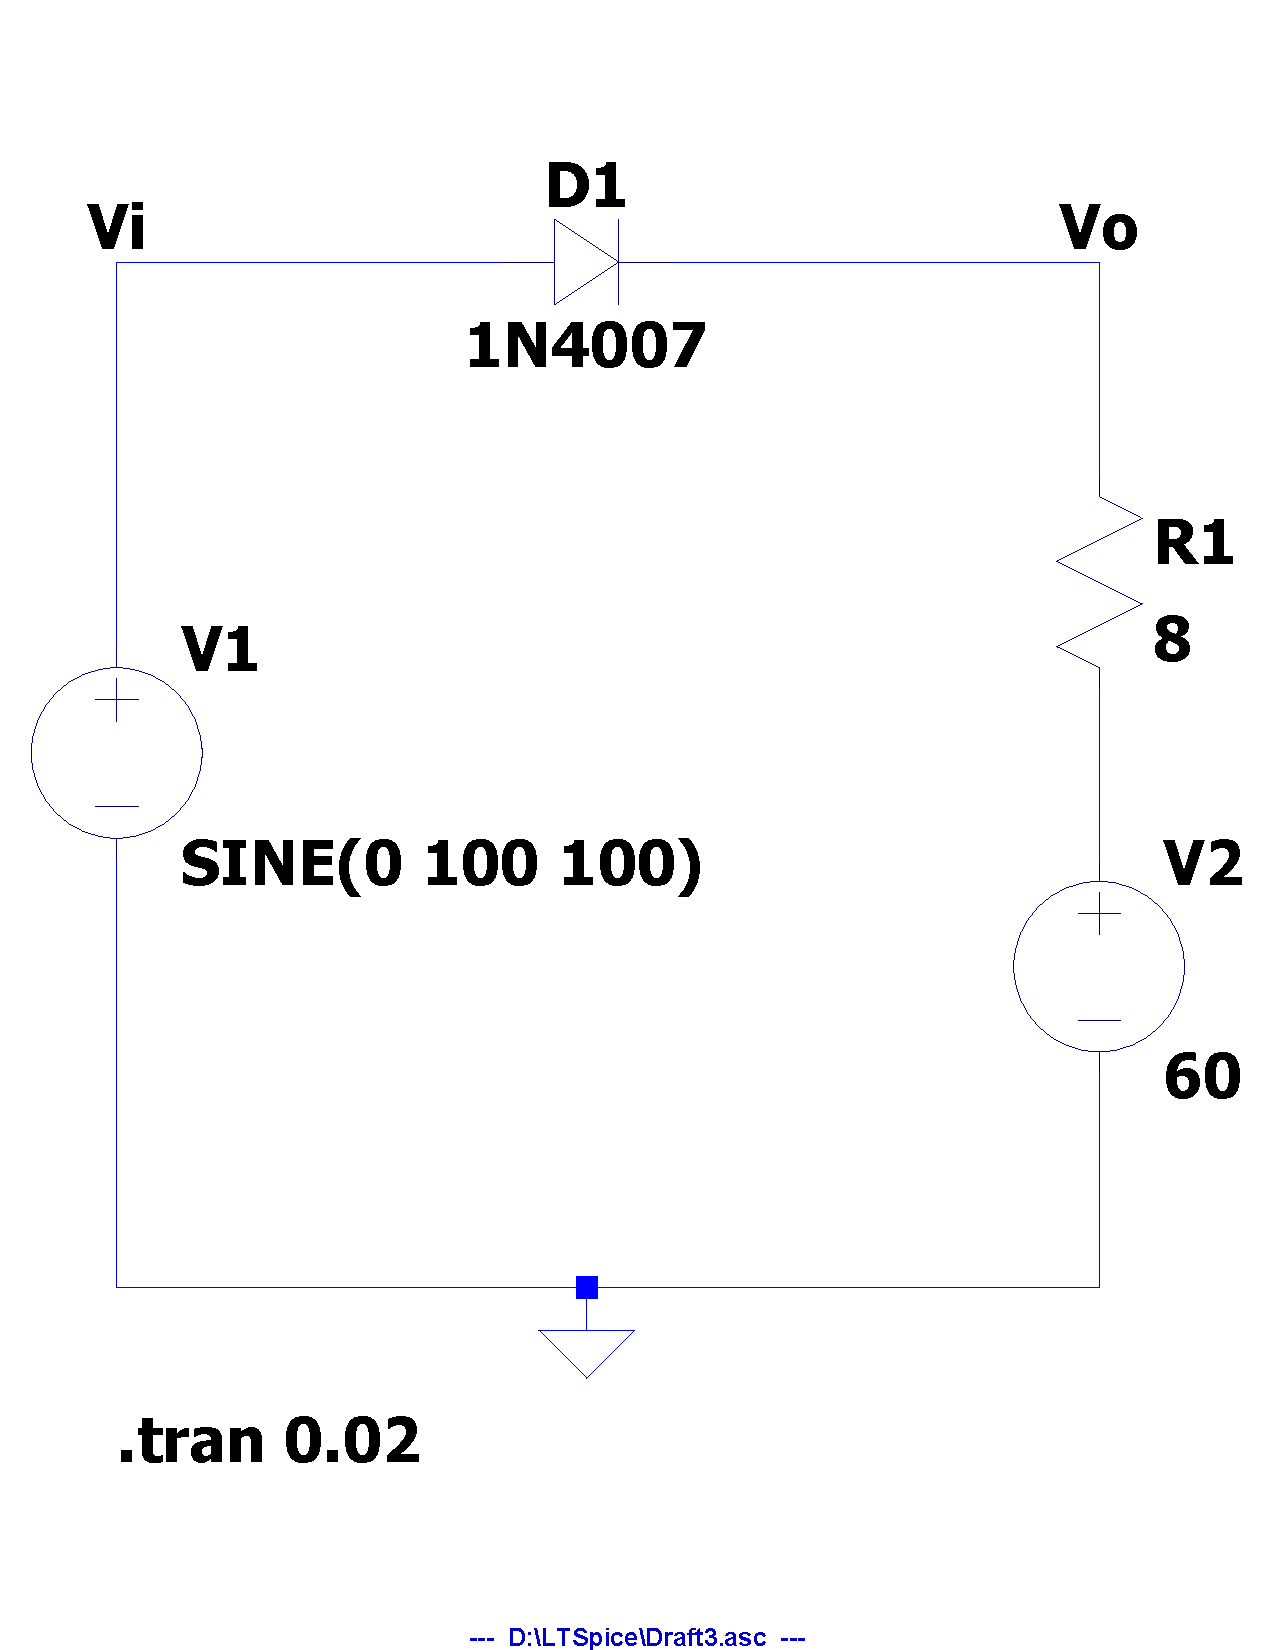
\includegraphics[clip, trim=0cm 4cm 0.5cm 1cm, scale=0.5]{circuito}
	\caption{}	
	\label{fig:figura3}
\end{figure}


\noindent Calculamos el valor de $\alpha$ en el cual el diodo comienza a conducir, para esto utilizamos la ecuación (4)
\begin{align}
	\alpha = \arcsin \left( \frac{60}{100} \right) = \qty{0.6435}{\radian} \nonumber
\end{align}

\noindent Utilizamos (5) para calcular el valor de $t_1$ en el cual el diodo comienza a conducir

\begin{align}
	t_1 = \frac{\alpha}{\omega} = \frac{0.6435}{2\pi \cdot 100} = \qty{1.024}{\milli \second} \nonumber
\end{align}

\noindent Calculamos el valor del tiempo en el cual el diodo deja de conducir
\begin{align}
	t_2 = \frac{\pi - \alpha}{\omega} = \frac{\pi - 0.6435}{2\pi \cdot 100} = \qty{3.97}{\milli \second} \nonumber
\end{align}

\noindent Utilizamos (17) para encontrar el valor del voltaje de salida promedio

\begin{align}
	V_{O(av)} = \left( \frac{1}{2\pi} \right) \left[ (2 \cdot 0.6435 + \pi)(60) + 2(100)\cos(0.6435) \right] = \qty{67.75}{\volt} \nonumber
\end{align}

\noindent Utilizamos (24) para encontrar el valor del voltaje de salida rms

\begin{align}
	V_{o(rms)} =\sqrt{\frac{1}{2\pi} \left[ (\pi + 2\alpha)(60)^2 + \frac{100^2}{2}\bigg(\pi - 2(0.6435) + \sin(2\cdot0.6435)\bigg) \right] } = \qty{69.11}{\volt} \nonumber
\end{align}

\end{document}